\documentclass{memo}
\usepackage{mathptm,mydef,myenv}
\usepackage[all]{xy}
\usepackage{graphicx}
%\usepackage{MinionPro}
\begin{document}
\small

\noindent{\large\bf{}Hadoop Distributed Filesystem}

\paragraph{Overview}
The Hadoop distributed filesystem (HDFS) was designed with the following
criteria in mind:
\bit
\w \bb{Very large files} Files are hundreds of MB, GB, or TB in size. Some
Hadoop clusters are running over PB of data. 
\w \bb{Streaming data access} HDFS is built around the idea that the most
efficient data processing pattern is a {\em write-once read-many-times\/}
pattern. A data is typically generated or copied from source, then various
analyses are performed on that dataset over time. Each analysis will involve a
large proportion of the dataset, so {\em turnaround time\/} is more important
than the {\em latency\/} in reading the first record.
\w \bb{Moving computation is cheaper than moving data} A computatino requested
by an application is much more efficient if it is executed near the data it
operates on. This is especially true when the size of the dataset is huge. 
\w \bb{Fault tolerance} Hadoop runs on {\em unreliable\/} commodity
hardware. So, fault tolerance is of utmost importance.
\eit

\paragraph{Hadoop blocks}
File system blocks are typically a few KB in size, while disk blocks are
normally 512 bytes. 
The HDFS block size is \bb{64 MB} by default. This minimizes the cost of
seeks compared to actual data transfer time. Also, it allows a file to be
larger than any signle physical disk and {\em fixed size\/} of blocks
simplifies filesystem management.

The Hadoop block is a unit of {\em replication\/} and typically three copies
of the same block is replicated in different machines.

\paragraph{Namenodes and datanodes}
An HDFS cluster has two types of node operating in a msater-worker pattern: a
{\em namenode} (the master) and a number of {\em datanodes} (workers). 
The \bb{namenode} manages the filesystem {\em namespace\/}. It maintains the
filesystem tree and the metadata for all the files and directories in the
tree. The \bb{datanode} store and retrieve blocks when they are told to (by
clients or the namenode). These nodes report back to the namenode periodically
with lists of blocks that they are storing. 

\paragraph{Namenode}
HDFS namespace is a hierarchy of files and directories. Each file and
directory are represented on the namenode using an {\em inode\/}, which
records attributes like permissions, modification and access times, disk space
quotas. The file content is split into large blocks (typically 64 or 128MB)
and each block is replicated at multiple datanodes. 

The namenode maintains the namespace tree and the \bb{mapping of file blocks to
datanodes} inside the RAM. This information is also stored {\em
  persistently\/} on the local disk 
in the form of two files: {\tt FsImage} and {\tt EditLog}. 

\paragraph{Namenode: Persistence of file system metadata}
The namenode uses a {\em transaction log\/} called the {\tt EditLog} to
persistently record every 
change that occurs to the filesystem metadata. For example, creating a new
file in HDFS causes the namenode to insert a record into the EditLog
indicating this. 

Also, the inode data and the list of blocks belonging to each file comprise
the metadata of the namespace called the {\tt FsImage}. The persistent record
of the image stored in the localhost's native file system is called a
\bb{checkpoint}. 

The namenode keeps an image of the entire filesystem namespace and file
{\tt Blockmap} {\em in memory\/}. When the namenode starts up, it reads the
{\tt FsImage} and {\tt EditLog} from disk, applies all the transactions from
the {\tt EditLog} to the in-memory representation of the {\tt FsImage}, and
flushes out this new version into a new {\tt FsImage} on disk. 

{\em Checkpointing} is a process which truncates the old {\tt EditLog} because
its transactions have been applied to the persistent {\tt FsImage}. 

\paragraph{Namenode: Fault tolerance}
Since the failure in the namenode corrupts the whole file system, it is
important to make the namenode resilient. For this, two methods are
used. The first way is to {\em back up} the files that make up the persistent
state of the filesystem metadata. Any change in metadata is stored (sometimes
to multiple copies) in an atomic and synchronous way.

Also, it's possible to run a {\em secondary namenode}, which periodiacally
merge the {\tt FsImage} and {\tt EditLog} to prevent the {\tt EditLog} from
becoming too large. 

\paragraph{Datanode}
Each block replica on a datanode is represented by two files in the local
host's native file system. The first file contains the data itself and the
second file is block's metadata including the checksums of the block data and
the block's {\em generation stamp\/}. 

During startup each datanode connects to the namenode and performs a {\bf
  handshake\/}. The purpose of handshaking is to verify the {\em namespace
  ID\/} and the {\em software version\/} of the datanode. If either does ontt
match that of the namenode the datanode automatically shuts down.

After the handshake, the datanode \bb{registers} with the namenode. Datanodes
persistently store their unique {\em storage IDs\/}. The storage ID is an
internal identifier of the datanode, which makes it recognizable even if it is
restarted with a different IP address or port. The storage ID is assigned to
the datanode by the namenode for the first time and this ID never changes
after that.

A datanode identifies the block replicas it possesses and sends a {\bf block
  report}, which contains the {\em block ID\/}, the {\em generation stamp\/},
and the length of each block replica the server hosts. This first block report
is sent right after the datande registration. Subsequent block reports are
sent every hour and provide the namenode with an up-to-data view of where
block replicas are located on the cluster.

\paragraph{Datanode: Fault tolerance}
The datanode sends \bb{hearbeats} to the namenode {\em every three seconds\/}
to confirm that the datanode is oeprating and the block replicas it hosts are
available. When namenode does not receive a hearbeat from a datanode, it
schedules creation of new replicas of the blocks on the dead datanode on other
datanodes. 




\paragraph{Hadoop filesystem types}
An HDFS implements the Java abstract class
\verb+org.apache.hadoop.fs.FileSystem+. There are several concrete
implementations:
\bit
\w \bb{Local file system}: a local filesystem for the client
\w \bb{HDFS}: Hadoop distributed filesystem to be worked with MapReduce
\w \bb{HAR}: A filesystem layered on another filesystem for archiving files
\w \bb{FTP}: a file system backed by FTP server
\w \bb{S3 (native or block-based)}: Amazon S3 filesystem
\w \bb{HFTP}, \bb{HSFTP}, \bb{FTP},\bb{KFS}
\eit

\paragraph{Anatomy of HDFS file read}
\begin{quote}
% jpg for pdflatex
%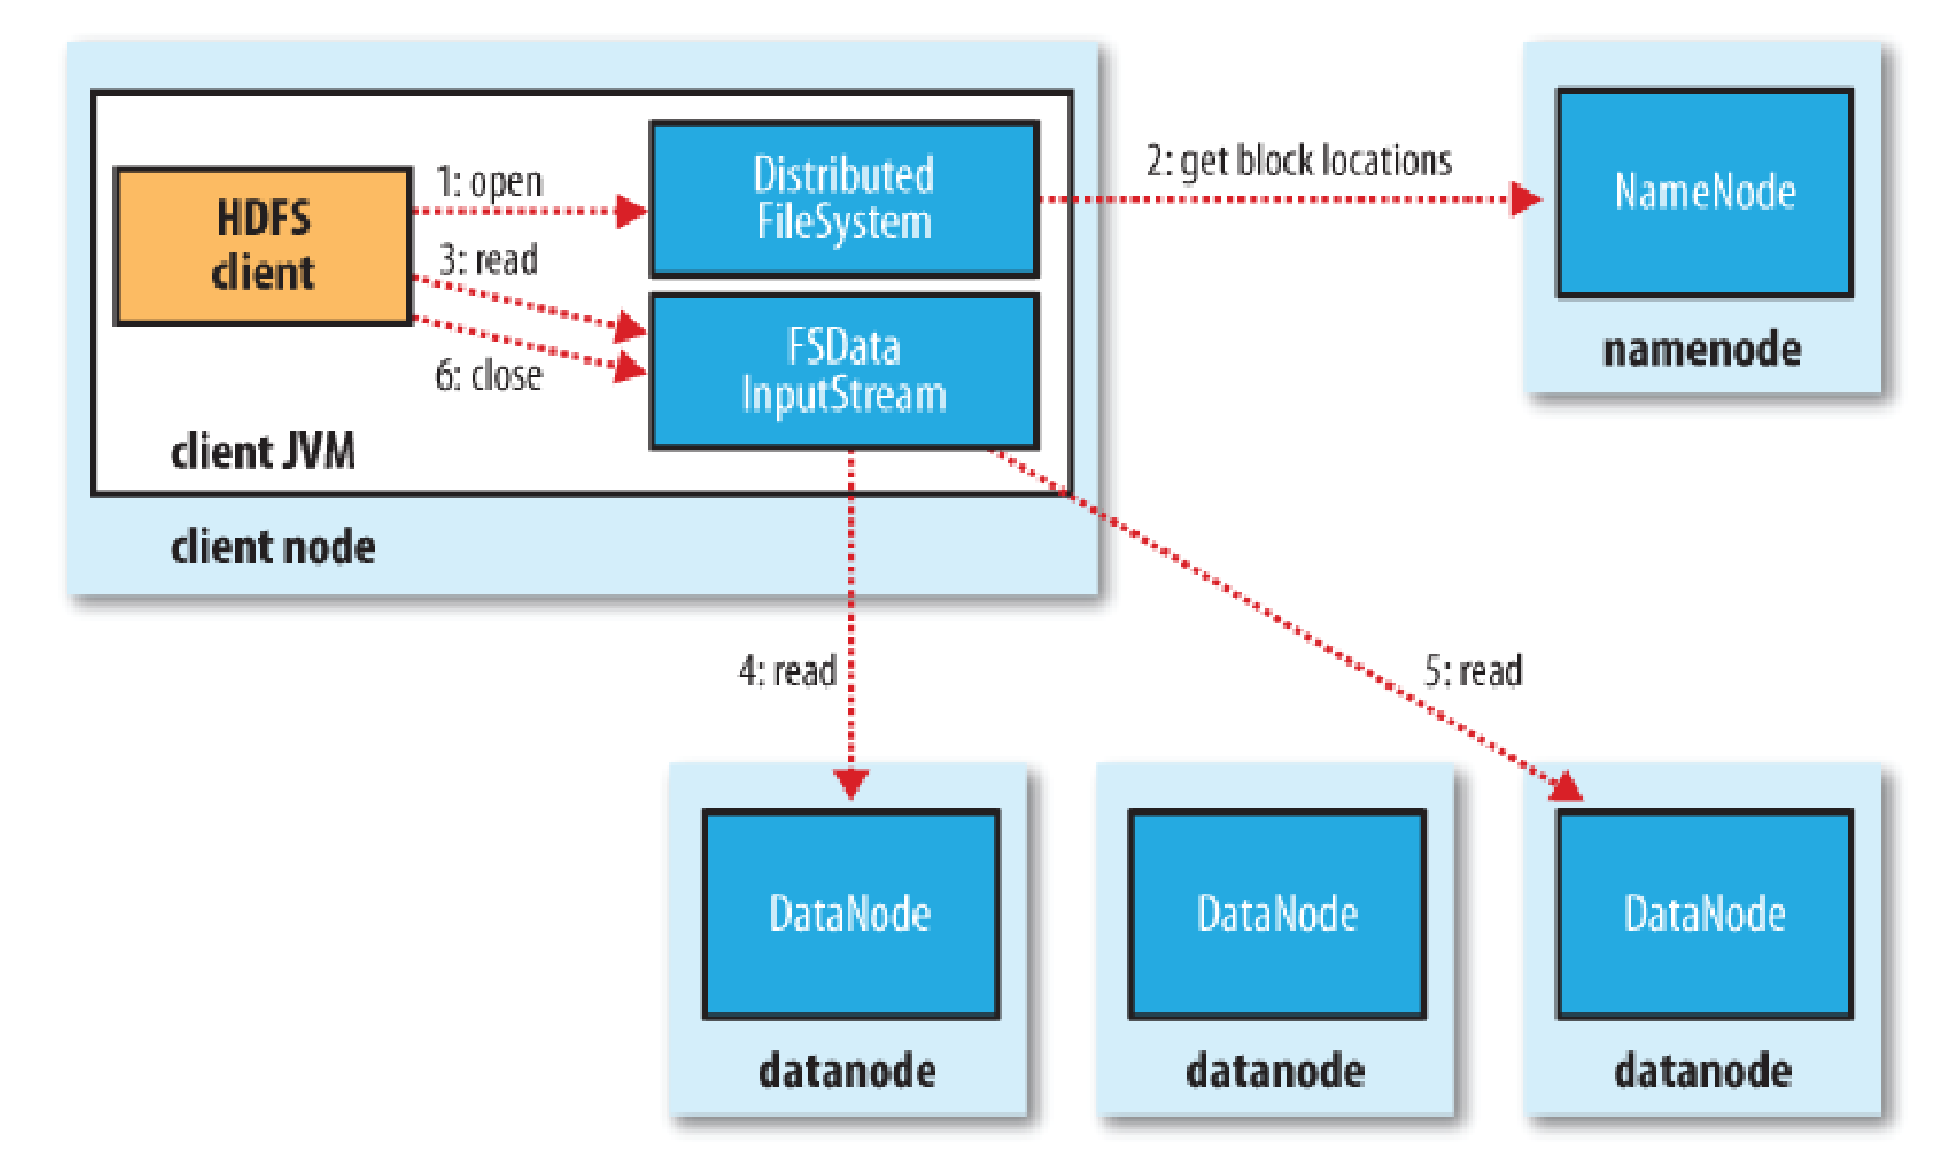
\includegraphics[scale=0.3]{fread.ps}
% ps for xdvi
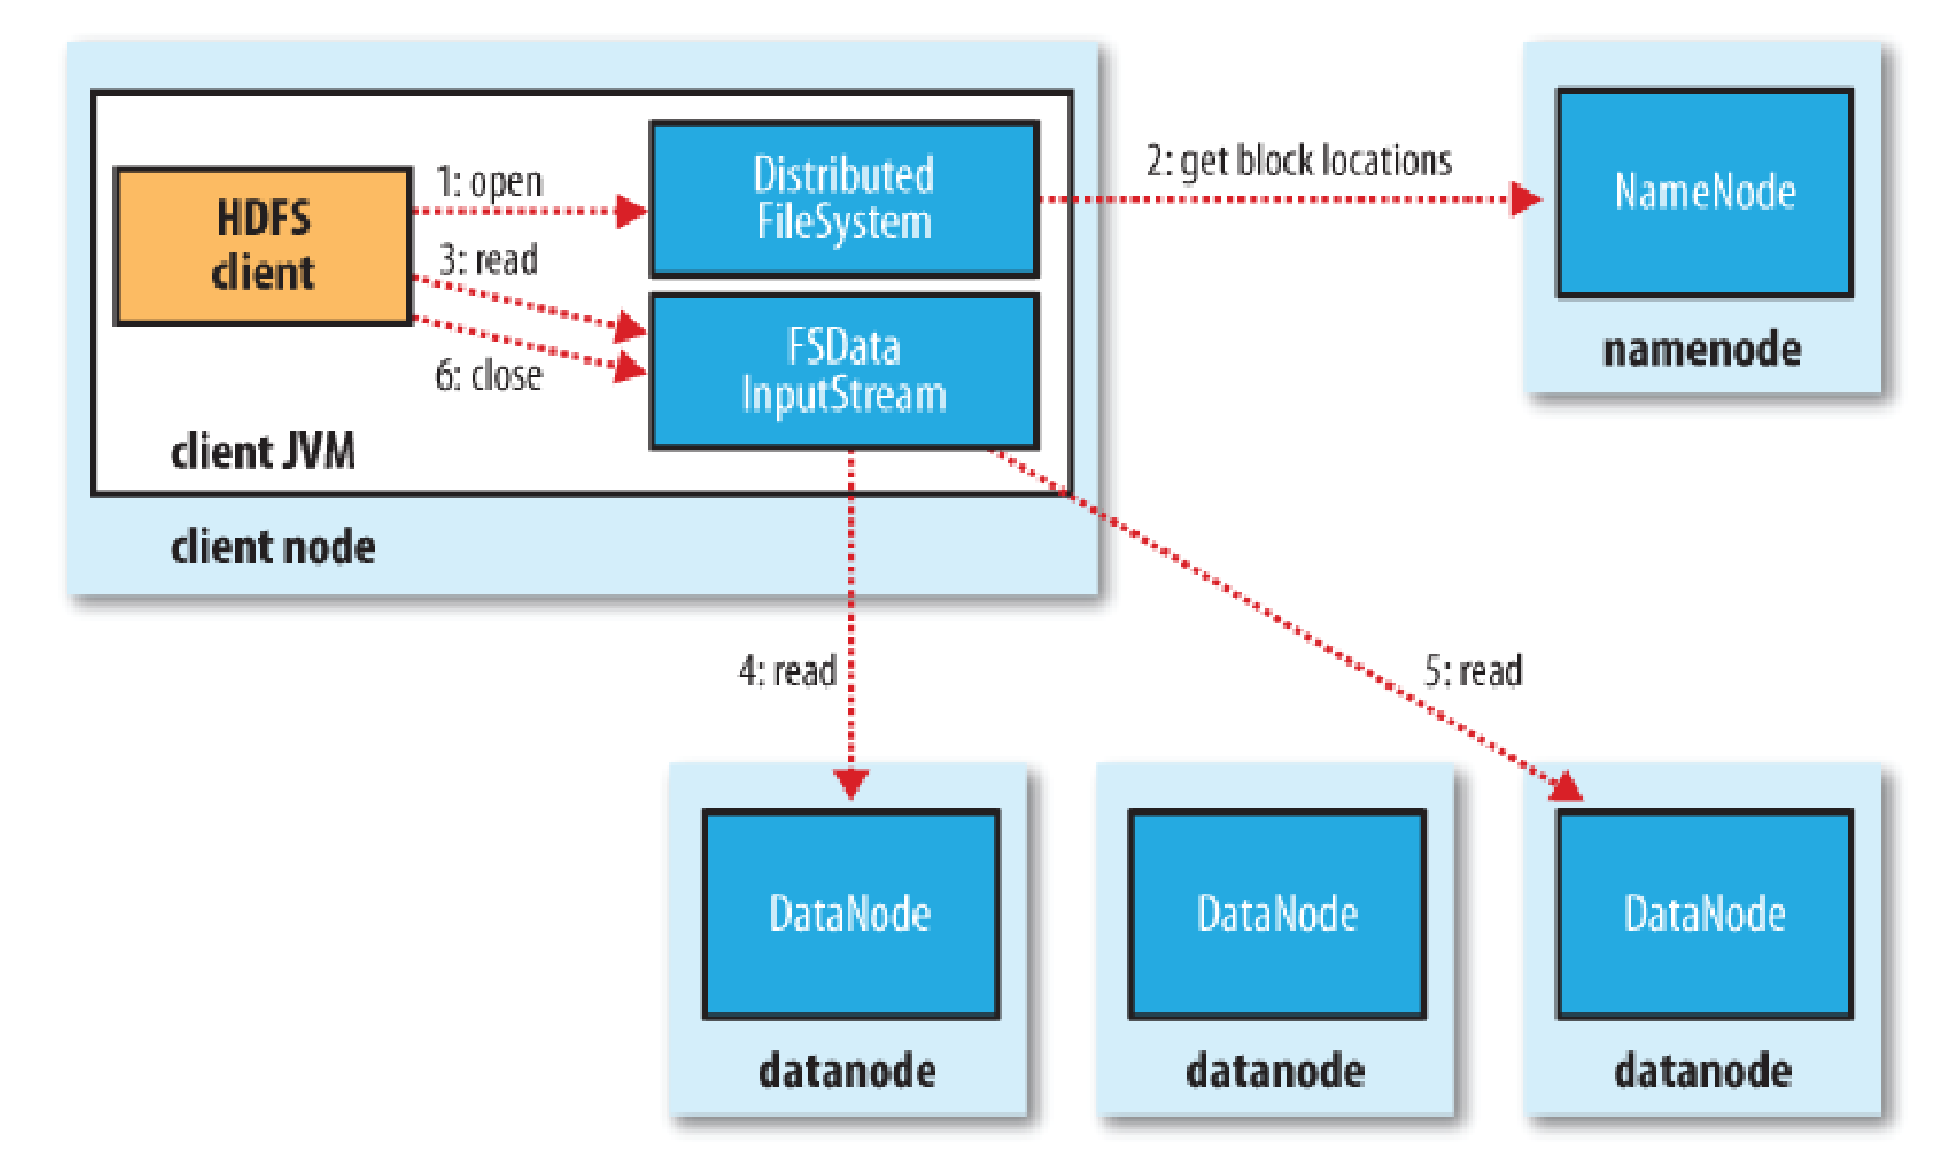
\includegraphics[scale=0.2]{fread.ps}
\end{quote}

\paragraph{Anatomy of HDFS file write}
\begin{quote}
% jpg for pdflatex
%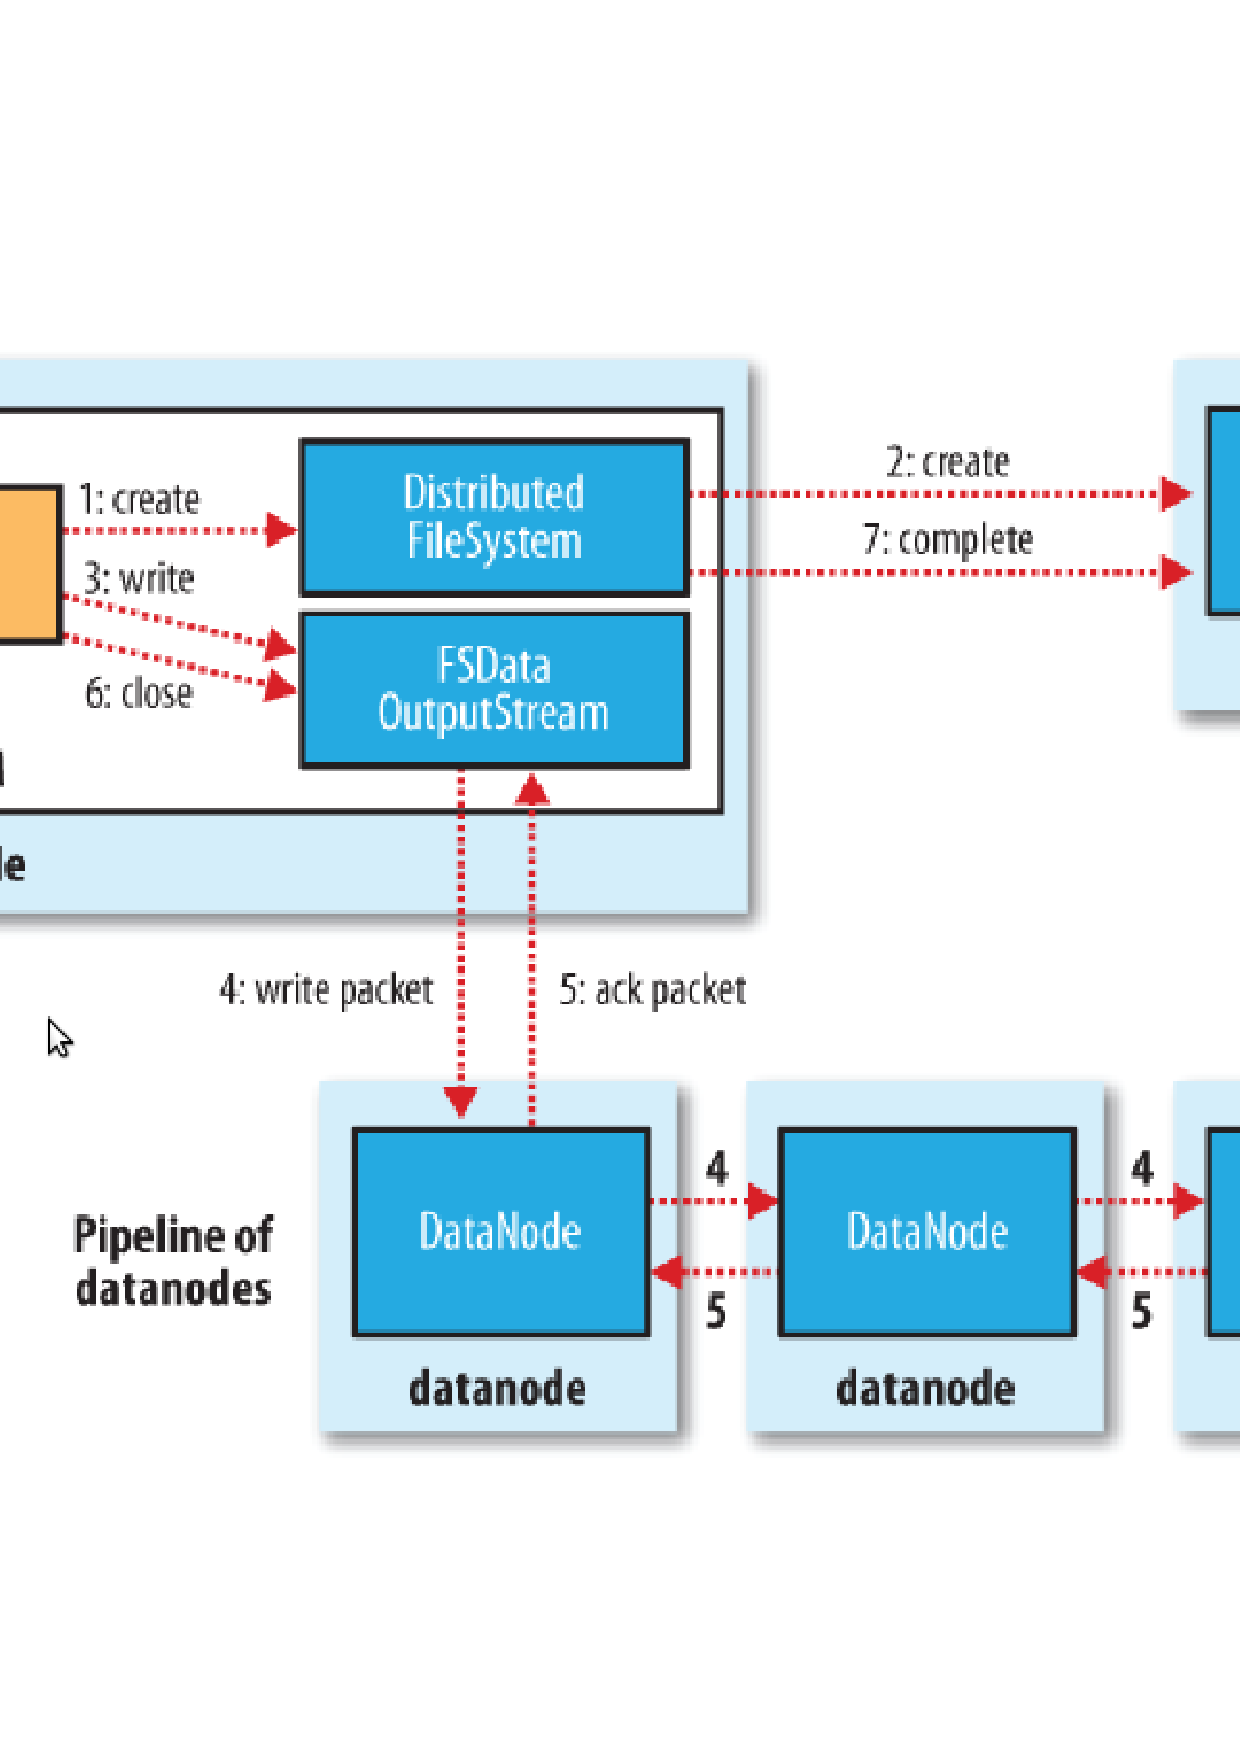
\includegraphics[scale=0.3]{fwrite.png}
% ps for xdvi
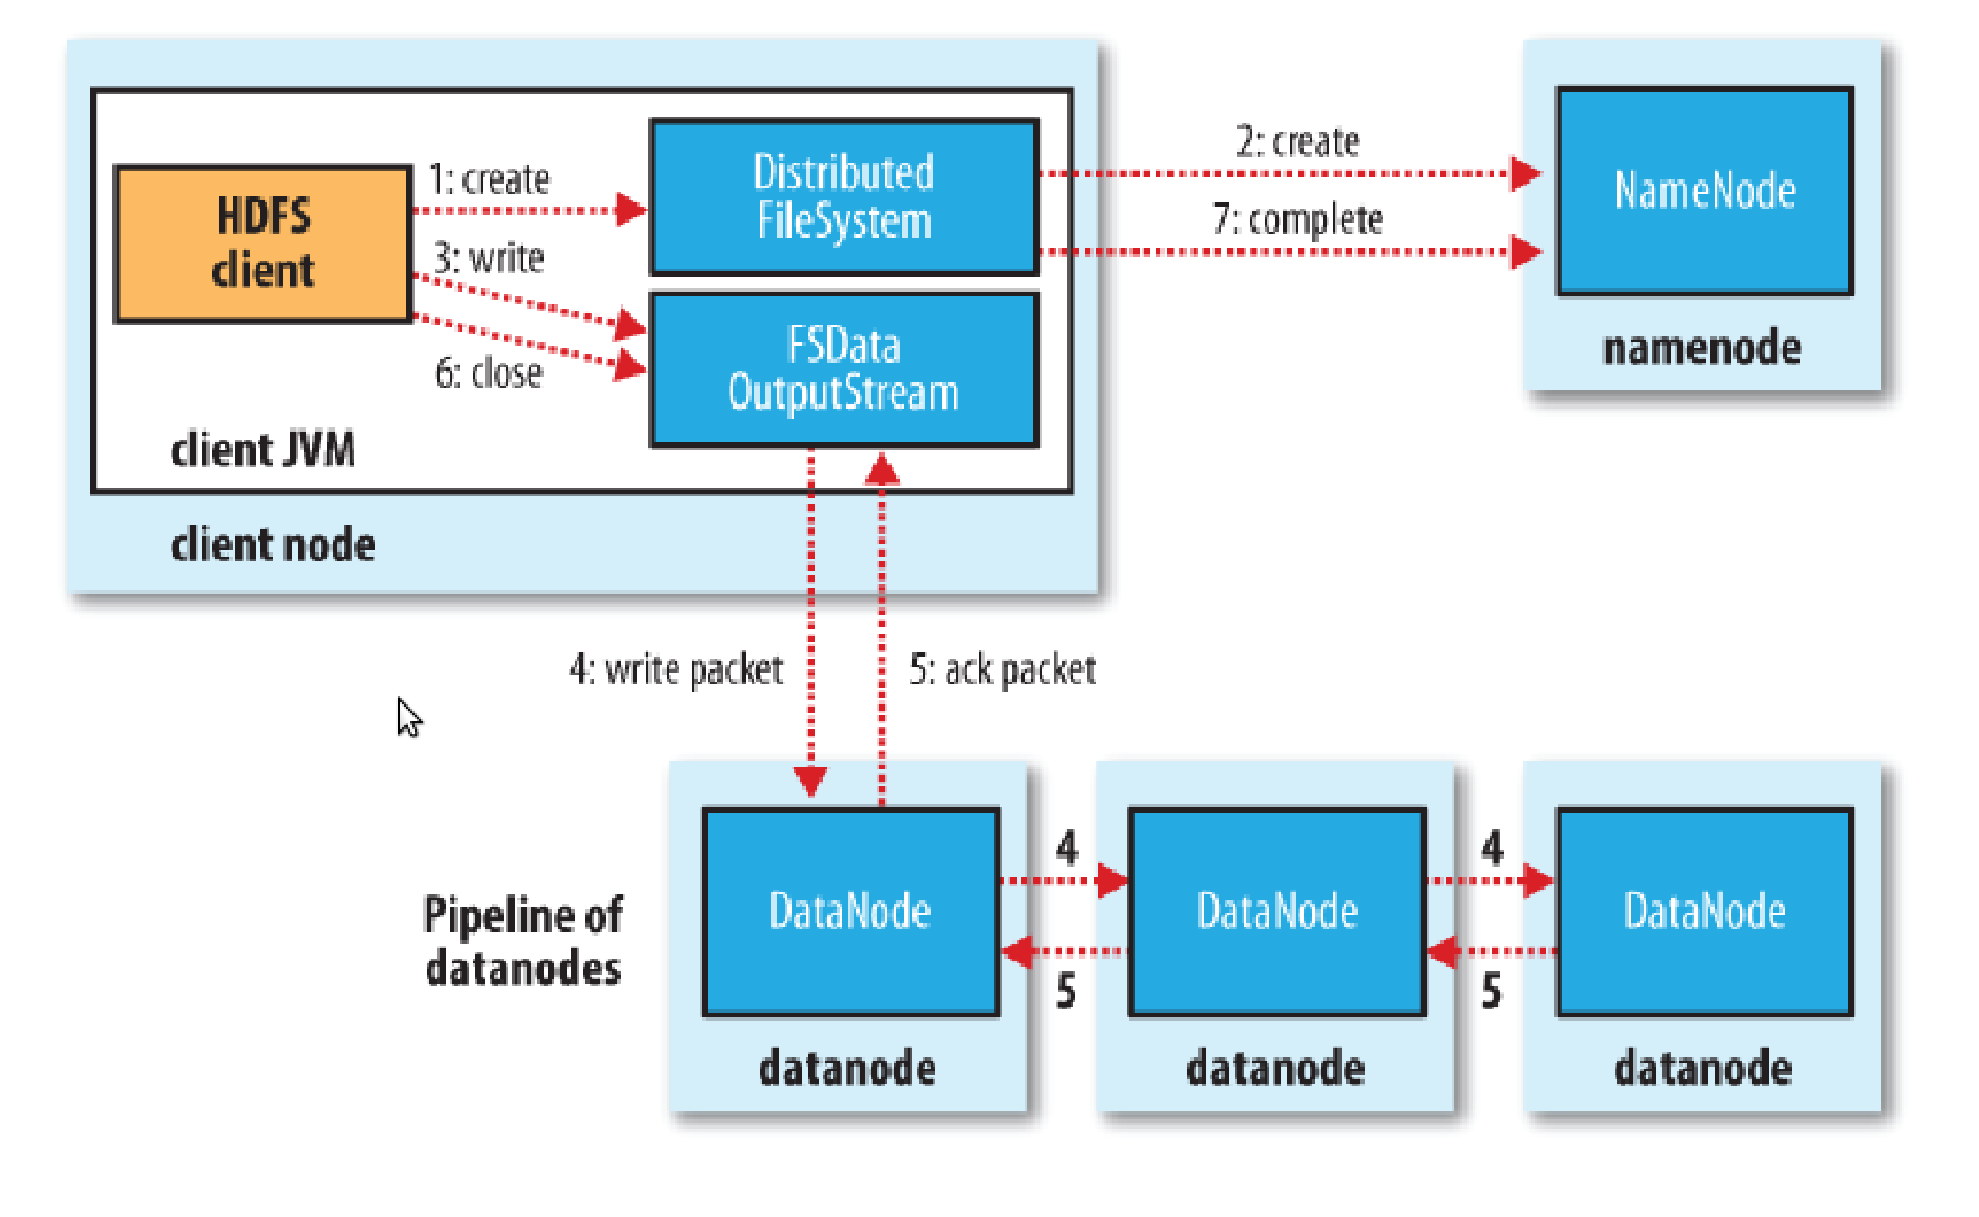
\includegraphics[scale=0.2]{fwrite.ps}
\end{quote}


\paragraph{Communication protocols}
All HDFS communication is layered on top of the TCP/IP protocol. A client
establishes a connection to a configurable TCP port on the namenode
machine. It taskes the \bb{ClientProtocol} with the namenode. The datanodes
talk to the namenode using the \bb{DataNodeProtocol}.  

\paragraph{File I/O}
When the HDFS client opens a file for writing, a \bb{lease} for the file is
granted keeping other clients from writing to the file. The writing client
{\em periodically renews} the lease by sending a {\em hearbeat} to the
namenode. When the file is closed, the lease is revoked.

\paragraph{Replica management}

\paragraph{Block placement}
For a large cluster, it may not be practical to connect all nodes in a flat
topology. A common practice is to spread the nodes {\em across multiple
  racks\/}.  Nodes of a rack share a switch, and rack switches are connected
by one or more core switches. 

\end{document}
